\label{sec:fixed}

\subsection{Dataset Preparation}

I did some some work to adapt \nolinkurl{mnist.py} to Python 3.
In order to get an appropriate scale, I did a search and got \autoref{fig:scale_pretest}, which shows the validation accuracy meets the requirement when the scale is around \(2^{16}\).
The validation accuracy reported by \nolinkurl{mnist.py} is as \autoref{fig:mnist-output}, where the validation error with fixed-point number is 18.98\%.

\begin{figure}[ht!]
    \centering
    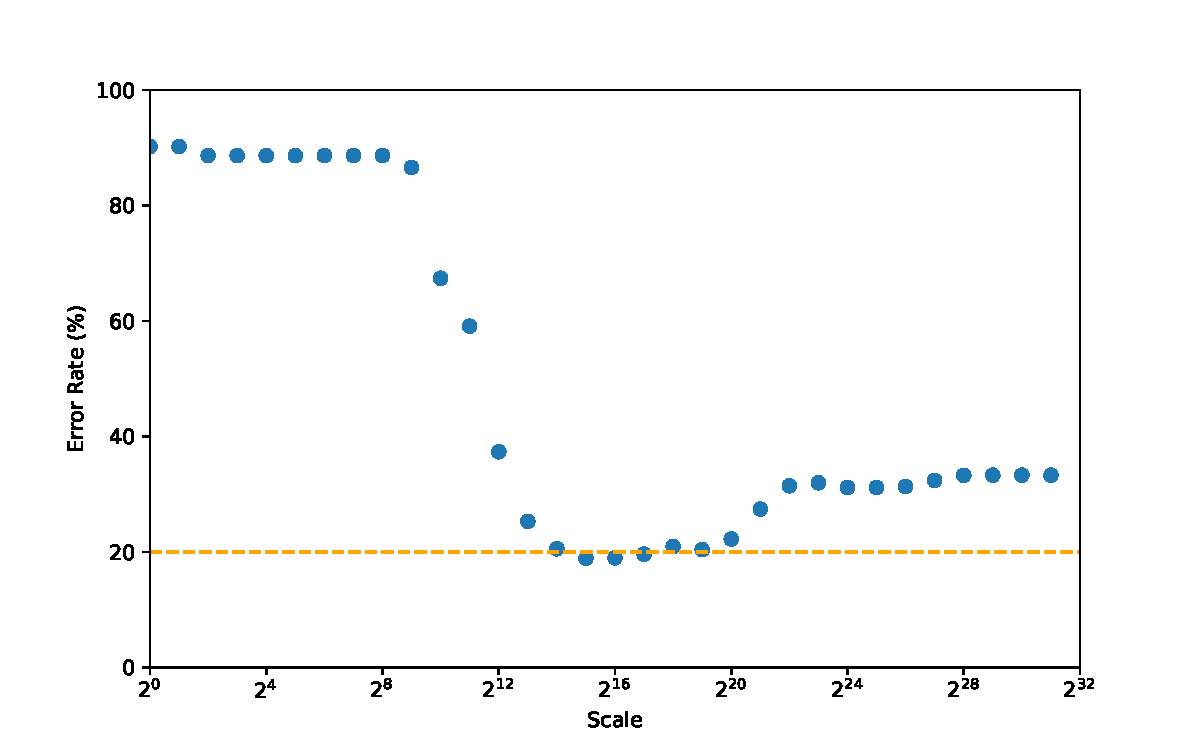
\includegraphics[scale=0.64]{images/scale_pretest.pdf}
    \caption{Misclassifications Rate with fixed point numbers under different scales}
    \label{fig:scale_pretest}
\end{figure}

\begin{figure}[ht!]
    \begin{minted}{console}
        $ python3 mnist.py
        Min/Max of coefficient values [-0.49227501415123354, 0.3931926418998524]
        Min/Max of intersect values [-0.12369156945342877, 0.2528140743366973]
        Misclassifications (float) = 14.05%
        Misclassifications (fixed) = 18.98%
    \end{minted}
    \caption{The output of \nolinkurl{mnist.py}}
    \label{fig:mnist-output}
\end{figure}

\subsection{Hardware Design}

\subsubsection{Timing}

The overall latency, as reported in \autoref{tab:fixed-latency}, is 386378 cycles for 8192 batches, which means 47.17 cycles for each input on average.
It is a 604.25x speedup over our baseline without auto pipelining.
The pipelined loop has an initiation interval of 1 cycle achieved, as reported in \autoref{tab:fixed-loop}.

\begin{table}[ht!]
    \centering
    \caption{Performance Estimates}\label{tab:fixed-latency}
    \begin{tabular}{ccccccc}
        \toprule
        \multicolumn{2}{c}{Latency (cycles) }   &
        \multicolumn{2}{c}{Latency (absolute) } &
        \multicolumn{2}{c}{Interval }           &
        \multirow{2}{*}{\makecell*{Pipeline                                                             \\ Type}}                 \\
        min                                     & max    & min      & max      & min    & max    &      \\
        \midrule
        386378                                  & 386378 & 3.864 ms & 3.864 ms & 386379 & 386379 & none \\
        \bottomrule
    \end{tabular}
\end{table}



\begin{table}
    \centering
    \begin{minipage}{0.48\linewidth}
        \centering
        \caption{Loop detail of the pipelined loop}\label{tab:fixed-loop}
        \begin{tabular}{ll|c}
            \toprule
                                &          & \verb+L1_L2+ \\
            \midrule
            Latency (cycles)    & min      & 1287                   \\
            Latency (cycles)    & max      & 1287                   \\
            Iteration Latency   &          & 9                      \\
            Initiation Interval & achieved & 1                      \\
            Initiation Interval & target   & 1                      \\
            Trip Count          &          & 1280                   \\
            Trip Count          &          & 1280                   \\
            Pipelined           &          & yes                    \\
            \bottomrule
        \end{tabular}
    \end{minipage}
    \begin{minipage}{0.48\linewidth}
        \centering
        \caption{Loop Latency of load, compute and store}
        \label{tab:fixed-loop-latency}
        \begin{tabular}{lcc}
            \toprule
            \multicolumn{1}{c}{\multirow{2}{*}{Loop Name}} & \multicolumn{2}{c}{Latency (cycles)}        \\
                                                           & min                                  & max  \\
            \midrule
            \verb+LOAD_INPUT_VITIS_LOOP_73_4+                         & 4096                                 & 4096 \\
            \verb+L1_L2+                         & 1287                                 & 1287 \\
            \verb+STORE_OUTPUT_VITIS_LOOP_106_6+                         & 642                                  & 642  \\
            \bottomrule
        \end{tabular}
    \end{minipage}
\end{table}



\subsubsection{Device Utilization}

The overall device utilization is reported as \autoref{tab:fixed-utilization}.
We have 128 multipliers implemented by LUT and 129 multiply-accumulate operator implemented on DSP.

\begin{table}[ht!]
    \centering
    \caption{Utilization Estimates Summary}\label{tab:fixed-utilization}
    \begin{tabular}{lrrrrr}
        \toprule
        \multicolumn{1}{c}{Name} & BRAM\_18K & DSP & FF     & LUT   & URAM \\
        \midrule
        DSP                      & -         & 129 & -      & -     & -    \\
        Expression               & -         & -   & 0      & 3967  & -    \\
        FIFO                     & -         & -   & -      & -     & -    \\
        Instance                 & 0         & 0   & 36     & 5247  & -    \\
        Memory                   & 260       & -   & 4160   & 517   & -    \\
        Multiplexer              & -         & -   & -      & 7513  & -    \\
        Register                 & -         & -   & 5633   & 128   & -    \\
        \midrule
        Total                    & 260       & 129 & 9829   & 17372 & 0    \\
        \midrule
        Available                & 280       & 220 & 106400 & 53200 & 0    \\
        \midrule
        Utilization (\%)         & 92        & 58  & 9      & 32    & 0    \\
        \bottomrule
    \end{tabular}
\end{table}

\subsection{Evaluation}

The measured system speedup over the fixed-point CPU implementation is 34.94x.
The measured misclassification rate on the 8k MNIST test sample is 19.96\% both on FPGA and on CPU.

\subsection{Reflection}
\label{sec:reflection}

The width of TDATA signal in AXI Stream interface is 64bit.
Each input data has 256 bytes, i.e., 32 words, and a tile of 128 inputs has 4096 words.
Our design, as reported in \autoref{tab:fixed-loop-latency}, took exactly 4096 cycles to load the 4096 words, but the following computation took only another 1287 cycles.
Thus I believe the design is memory-bandwidth limited.
That is, if we can load more data at a single cycle, we can achieve a higher overall throughput.

% A further inspection shows that the load-compute-store workflow is not fully pipelined.
% That is because we cannot pipeline at L1, which will lead to resource utilization exceeding the budget with the current parameter.
% A potential optimization could be reducing the tile size so that the three inner loops can be merged and pipelined.
